\chapter{要素技術}
\section{メトリックマップに基づくナビゲーション}
メトリックマップに基づくナビゲーションについて説明する.
ナビゲーションを行うためには, LiDAR やオドメトリなどのセンサとメトリックマップを活用し,自己位置推定や経路計画を行うことが必要である..
はじめに自己位置推定を行い,ロボットが地図上のどこに位置しているかを特定する.
これには, LiDAR やオドメトリデータなどのセンサ情報を利用したアルゴリズムである, AMCL (Adaptive Monte Carlo Localization)などを活用する.
次に,推定した自己位置から目的地までの最適な経路を計画し,経路に基づいてロボットを制御する.
メトリックマップに基づくナビゲーションでは,事前に取得した環境情報を活用できるという利点がある.
\figref{fig:nav}にメトリックマップに基づくナビゲーションの例を示す.
本論文ではメトリックマップに基づくナビゲーションにより計算される目標角速度を教師として模倣学習を行う.

\begin{figure}[htbp]
  \centering
  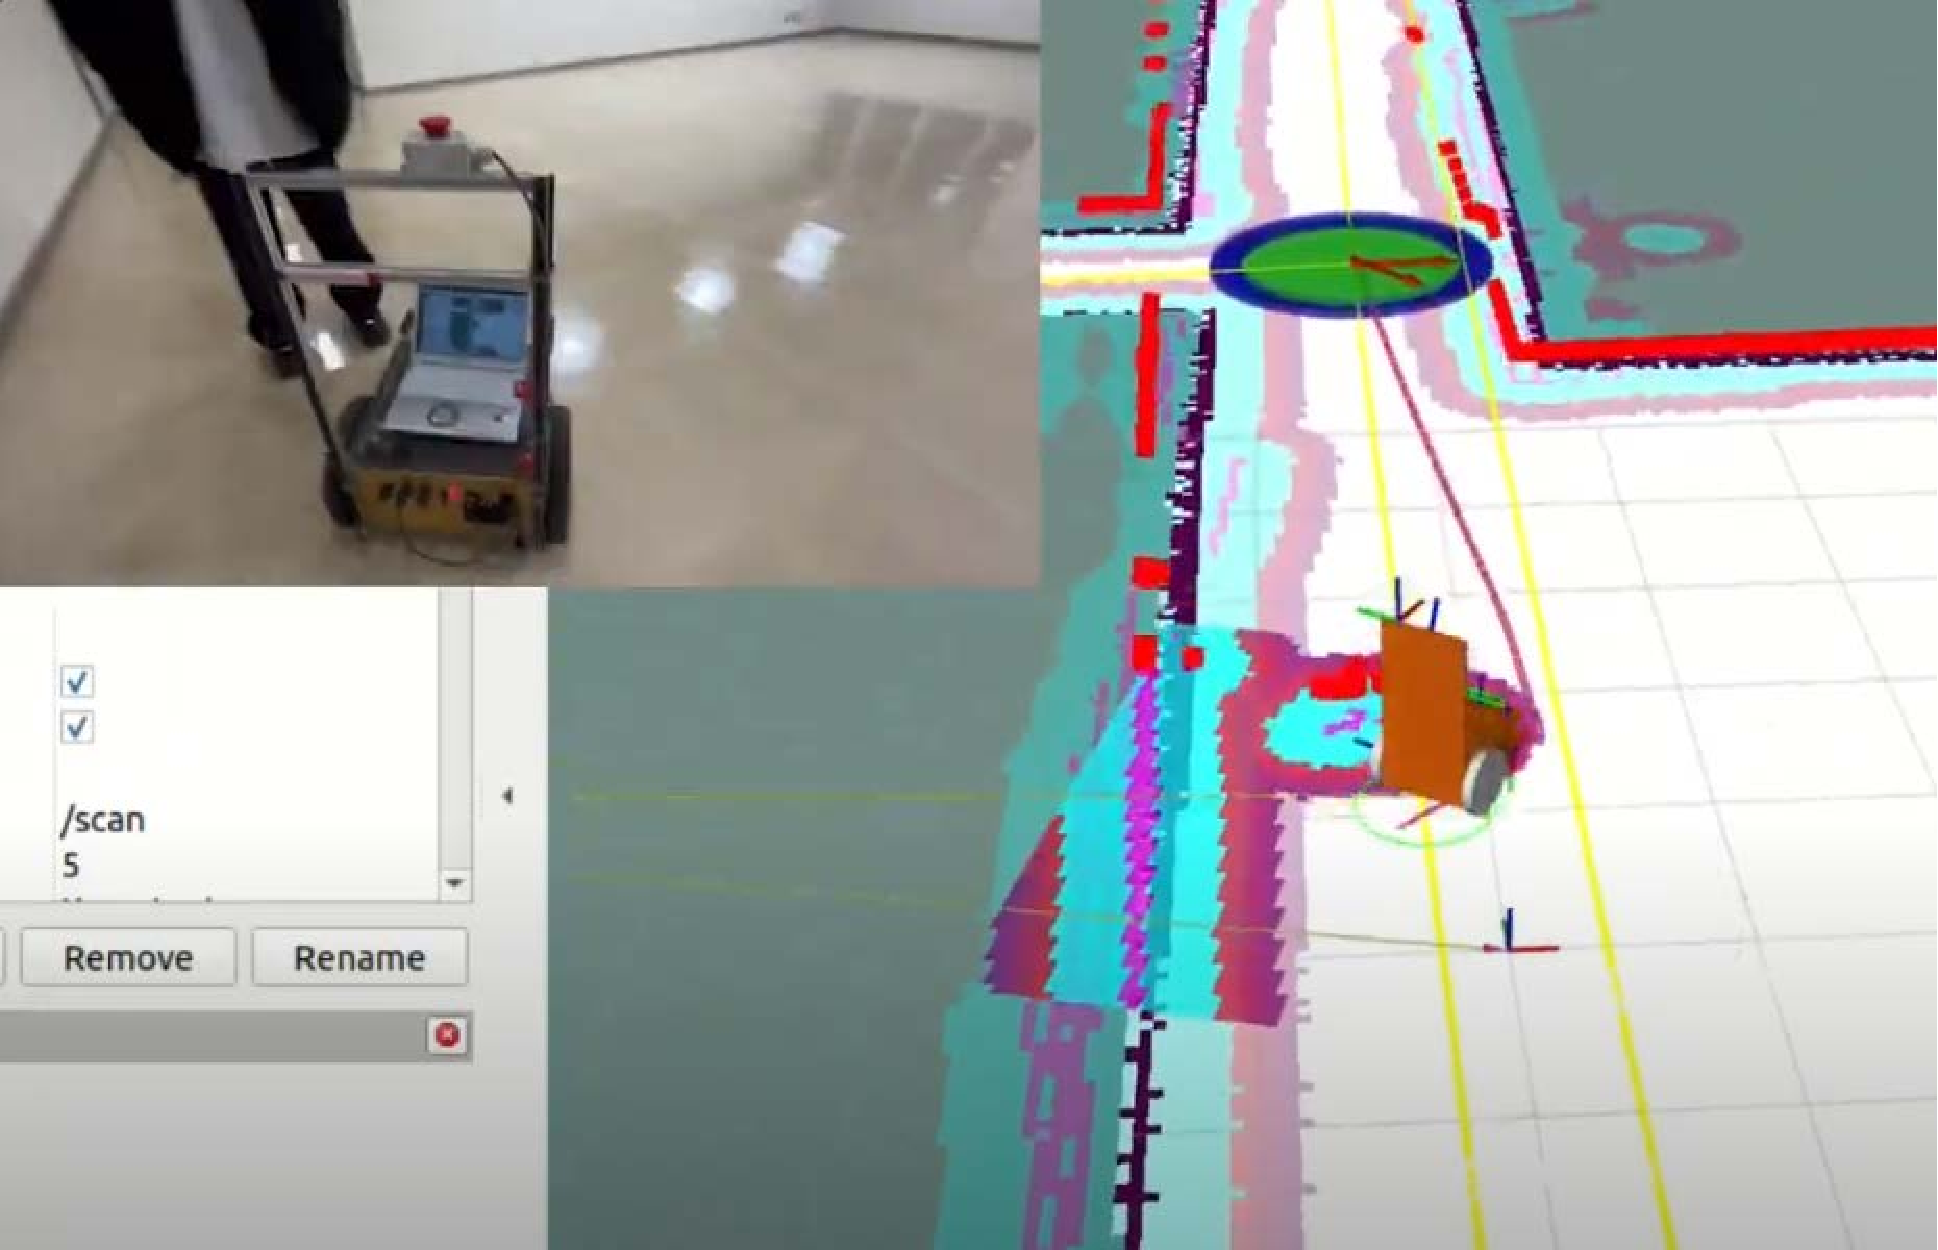
\includegraphics[width=130mm]{images/pdf/other/nav.pdf}
  \caption{Navigation based on metric map}
  \label{fig:nav}
\end{figure}